% 2005 年上海文科卷第 12 题：两个拼合示意
\begin{tikzpicture}[scale=0.78]
  % 原页并排重复的两幅棱柱拼合示意；尺寸标注不代表绘图比例。
  \foreach \dx in {0,5} {
    \begin{scope}[shift={ (\dx,0) }]
      \coordinate (A) at (0,0);
      \coordinate (B) at (3.15,0);
      \coordinate (C) at (3.15,1.05);
      \coordinate (D) at (0,1.05);
      \coordinate (E) at (2.10,1.62);
      \coordinate (F) at (2.10,0.57);

      % 可见棱与隐藏棱
      \draw (A)--(B)--(C)--(D)--(E)--(C);
      \draw (D)--(A);
      \draw[dashed] (E)--(F);
      \draw[dashed] (A)--(F)--(B);

      % 尺寸标注
      \node[left] at (-0.15,0.53) {$\dfrac{2}{a}$};
      \node[below] at (1.58,-0.18) {$5a$};
      \node[below,rotate=-29] at (2.65,0.24) {$3a$};
      \node[above,rotate=15] at (1.12,0.23) {$4a$};
    \end{scope}
  }
\end{tikzpicture}
